\documentclass{standalone}
\usepackage{tikz}
\usetikzlibrary{patterns, positioning}


\begin{document}
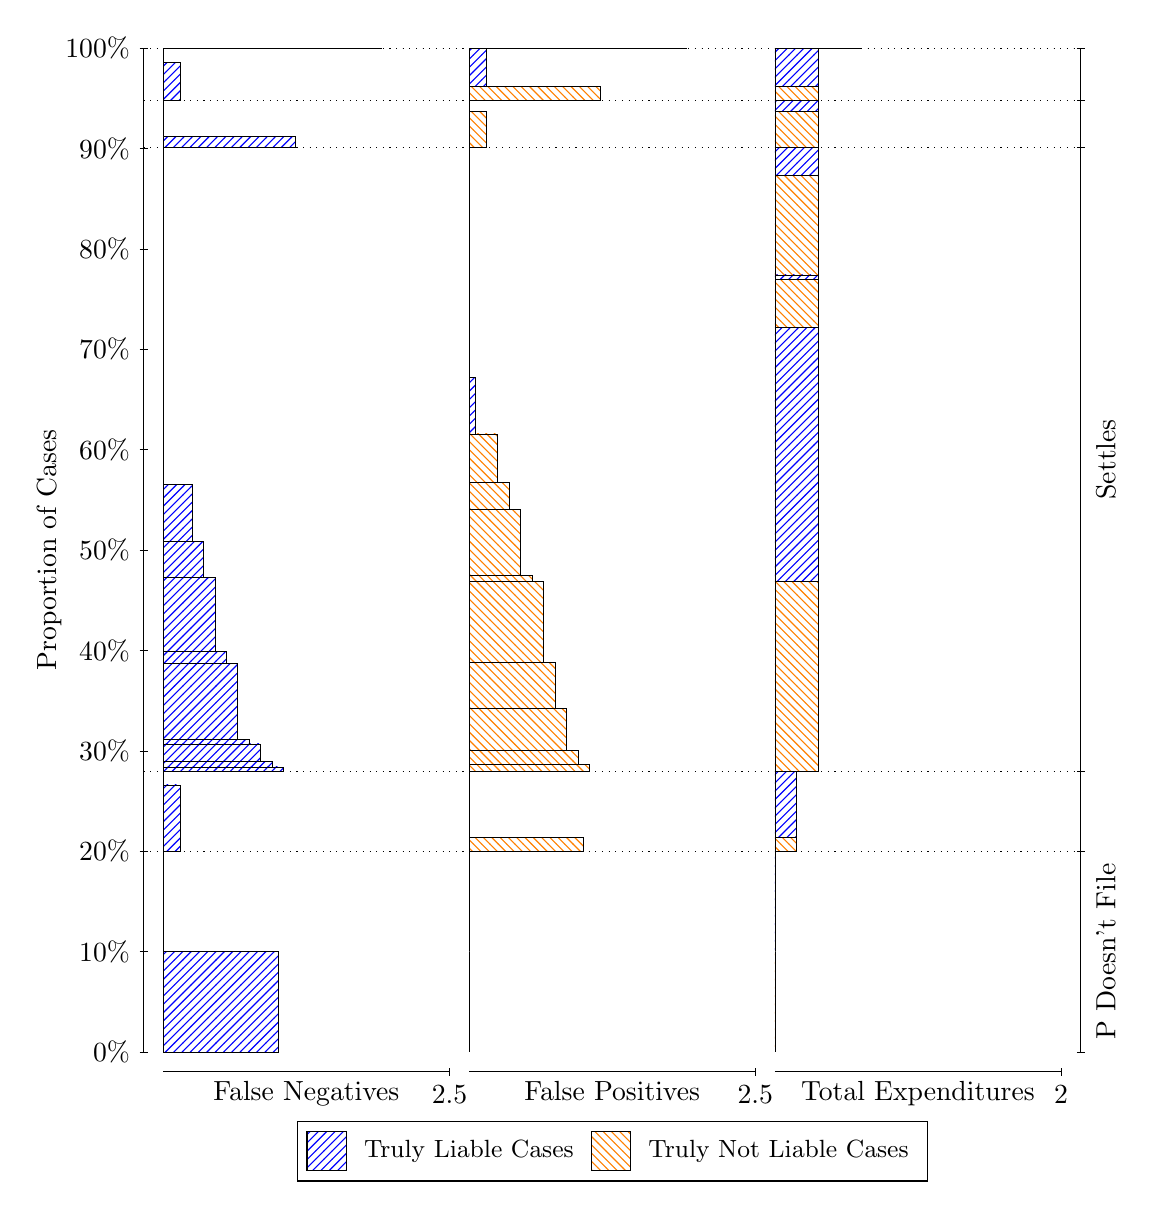
\begin{tikzpicture}
\draw[black, very thin] (1.5,1.75) -- (1.5,14.5);
\node[rotate=90, text=black, anchor=center] at (0.3, 8.125) {Proportion of Cases};
\draw[black, very thin] (1.45,1.75) -- (1.55,1.75);
\node[text=black, anchor=east] at (1.45, 1.75) {0\%};
\draw[black, very thin] (1.45,3.025) -- (1.55,3.025);
\node[text=black, anchor=east] at (1.45, 3.025) {10\%};
\draw[black, very thin] (1.45,4.3) -- (1.55,4.3);
\node[text=black, anchor=east] at (1.45, 4.3) {20\%};
\draw[black, very thin] (1.45,5.575) -- (1.55,5.575);
\node[text=black, anchor=east] at (1.45, 5.575) {30\%};
\draw[black, very thin] (1.45,6.85) -- (1.55,6.85);
\node[text=black, anchor=east] at (1.45, 6.85) {40\%};
\draw[black, very thin] (1.45,8.125) -- (1.55,8.125);
\node[text=black, anchor=east] at (1.45, 8.125) {50\%};
\draw[black, very thin] (1.45,9.4) -- (1.55,9.4);
\node[text=black, anchor=east] at (1.45, 9.4) {60\%};
\draw[black, very thin] (1.45,10.675) -- (1.55,10.675);
\node[text=black, anchor=east] at (1.45, 10.675) {70\%};
\draw[black, very thin] (1.45,11.95) -- (1.55,11.95);
\node[text=black, anchor=east] at (1.45, 11.95) {80\%};
\draw[black, very thin] (1.45,13.225) -- (1.55,13.225);
\node[text=black, anchor=east] at (1.45, 13.225) {90\%};
\draw[black, very thin] (1.45,14.5) -- (1.55,14.5);
\node[text=black, anchor=east] at (1.45, 14.5) {100\%};

\draw[black, very thin] (13.4,1.75) -- (13.4,14.5);
\draw[black, very thin] (13.35,1.75) -- (13.45,1.75);
\node[anchor=west] at (13.35, 1.75) {};
\draw[black, very thin] (13.35,4.3) -- (13.45,4.3);
\node[anchor=west] at (13.35, 4.3) {};
\draw[black, very thin] (13.35,5.316) -- (13.45,5.316);
\node[anchor=west] at (13.35, 5.316) {};
\draw[black, very thin] (13.35,13.236) -- (13.45,13.236);
\node[anchor=west] at (13.35, 13.236) {};
\draw[black, very thin] (13.35,13.836) -- (13.45,13.836);
\node[anchor=west] at (13.35, 13.836) {};
\draw[black, very thin] (13.35,14.494) -- (13.45,14.494);
\node[anchor=west] at (13.35, 14.494) {};
\draw[black, very thin] (13.35,14.497) -- (13.45,14.497);
\node[anchor=west] at (13.35, 14.497) {};
\draw[black, very thin] (13.35,14.5) -- (13.45,14.5);
\node[anchor=west] at (13.35, 14.5) {};

\draw[black, very thin, pattern color=blue, pattern=north east lines] (1.75,1.75) rectangle (3.2033,3.025);
\draw[black, very thin, pattern color=orange, pattern=north west lines] (1.75,3.025) rectangle (1.75,4.3);
\draw[black, very thin, pattern color=blue, pattern=north east lines] (1.75,4.3) rectangle (1.968,5.1412);
\draw[black, very thin, pattern color=orange, pattern=north west lines] (1.75,5.1412) rectangle (1.75,5.316);
\draw[black, very thin, pattern color=blue, pattern=north east lines] (1.75,5.316) rectangle (3.276,5.3693);
\draw[black, very thin, pattern color=blue, pattern=north east lines] (1.75,5.3693) rectangle (3.1307,5.4452);
\draw[black, very thin, pattern color=blue, pattern=north east lines] (1.75,5.4452) rectangle (2.9853,5.6624);
\draw[black, very thin, pattern color=blue, pattern=north east lines] (1.75,5.6624) rectangle (2.84,5.7215);
\draw[black, very thin, pattern color=blue, pattern=north east lines] (1.75,5.7215) rectangle (2.6947,6.6899);
\draw[black, very thin, pattern color=blue, pattern=north east lines] (1.75,6.6899) rectangle (2.5493,6.8325);
\draw[black, very thin, pattern color=blue, pattern=north east lines] (1.75,6.8325) rectangle (2.404,7.7777);
\draw[black, very thin, pattern color=blue, pattern=north east lines] (1.75,7.7777) rectangle (2.2587,8.2303);
\draw[black, very thin, pattern color=blue, pattern=north east lines] (1.75,8.2303) rectangle (2.1133,8.9535);
\draw[black, very thin, pattern color=orange, pattern=north west lines] (1.75,8.9535) rectangle (1.75,13.236);
\draw[black, very thin, pattern color=blue, pattern=north east lines] (1.75,13.236) rectangle (3.4213,13.377);
\draw[black, very thin, pattern color=orange, pattern=north west lines] (1.75,13.377) rectangle (1.75,13.836);
\draw[black, very thin, pattern color=blue, pattern=north east lines] (1.75,13.836) rectangle (1.968,14.314);
\draw[black, very thin, pattern color=orange, pattern=north west lines] (1.75,14.314) rectangle (1.75,14.494);
\draw[black, very thin, pattern color=blue, pattern=north east lines] (1.75,14.494) rectangle (4.5113,14.495);
\draw[black, very thin, pattern color=orange, pattern=north west lines] (1.75,14.495) rectangle (1.75,14.497);
\draw[black, very thin, pattern color=orange, pattern=north west lines] (1.75,14.497) rectangle (1.75,14.498);
\draw[black, very thin, pattern color=blue, pattern=north east lines] (1.75,14.498) rectangle (1.75,14.5);
\draw[black, very thin, pattern color=orange, pattern=north west lines] (5.6333,1.75) rectangle (5.6333,3.025);
\draw[black, very thin, pattern color=blue, pattern=north east lines] (5.6333,3.025) rectangle (5.6333,4.3);
\draw[black, very thin, pattern color=orange, pattern=north west lines] (5.6333,4.3) rectangle (7.0867,4.4749);
\draw[black, very thin, pattern color=blue, pattern=north east lines] (5.6333,4.4749) rectangle (5.6333,5.316);
\draw[black, very thin, pattern color=orange, pattern=north west lines] (5.6333,5.316) rectangle (7.1593,5.4059);
\draw[black, very thin, pattern color=orange, pattern=north west lines] (5.6333,5.4059) rectangle (7.014,5.5796);
\draw[black, very thin, pattern color=orange, pattern=north west lines] (5.6333,5.5796) rectangle (6.8687,6.1155);
\draw[black, very thin, pattern color=orange, pattern=north west lines] (5.6333,6.1155) rectangle (6.7233,6.7003);
\draw[black, very thin, pattern color=orange, pattern=north west lines] (5.6333,6.7003) rectangle (6.578,7.7234);
\draw[black, very thin, pattern color=orange, pattern=north west lines] (5.6333,7.7234) rectangle (6.4327,7.8033);
\draw[black, very thin, pattern color=orange, pattern=north west lines] (5.6333,7.8033) rectangle (6.2873,8.6396);
\draw[black, very thin, pattern color=orange, pattern=north west lines] (5.6333,8.6396) rectangle (6.142,8.9877);
\draw[black, very thin, pattern color=orange, pattern=north west lines] (5.6333,8.9877) rectangle (5.9967,9.5985);
\draw[black, very thin, pattern color=blue, pattern=north east lines] (5.6333,9.5985) rectangle (5.706,10.322);
\draw[black, very thin, pattern color=blue, pattern=north east lines] (5.6333,10.322) rectangle (5.6333,13.236);
\draw[black, very thin, pattern color=orange, pattern=north west lines] (5.6333,13.236) rectangle (5.8513,13.695);
\draw[black, very thin, pattern color=blue, pattern=north east lines] (5.6333,13.695) rectangle (5.6333,13.836);
\draw[black, very thin, pattern color=orange, pattern=north west lines] (5.6333,13.836) rectangle (7.3047,14.017);
\draw[black, very thin, pattern color=blue, pattern=north east lines] (5.6333,14.017) rectangle (5.8513,14.494);
\draw[black, very thin, pattern color=orange, pattern=north west lines] (5.6333,14.494) rectangle (5.6333,14.496);
\draw[black, very thin, pattern color=blue, pattern=north east lines] (5.6333,14.496) rectangle (5.6333,14.497);
\draw[black, very thin, pattern color=orange, pattern=north west lines] (5.6333,14.497) rectangle (8.3947,14.498);
\draw[black, very thin, pattern color=blue, pattern=north east lines] (5.6333,14.498) rectangle (6.9413,14.5);
\draw[black, very thin, pattern color=orange, pattern=north west lines] (9.5167,1.75) rectangle (9.5167,3.025);
\draw[black, very thin, pattern color=blue, pattern=north east lines] (9.5167,3.025) rectangle (9.5167,4.3);
\draw[black, very thin, pattern color=orange, pattern=north west lines] (9.5167,4.3) rectangle (9.7892,4.4749);
\draw[black, very thin, pattern color=blue, pattern=north east lines] (9.5167,4.4749) rectangle (9.7892,5.316);
\draw[black, very thin, pattern color=orange, pattern=north west lines] (9.5167,5.316) rectangle (10.062,7.7234);
\draw[black, very thin, pattern color=blue, pattern=north east lines] (9.5167,7.7234) rectangle (10.062,10.955);
\draw[black, very thin, pattern color=orange, pattern=north west lines] (9.5167,10.955) rectangle (10.062,11.566);
\draw[black, very thin, pattern color=blue, pattern=north east lines] (9.5167,11.566) rectangle (10.062,11.62);
\draw[black, very thin, pattern color=orange, pattern=north west lines] (9.5167,11.62) rectangle (10.062,12.884);
\draw[black, very thin, pattern color=blue, pattern=north east lines] (9.5167,12.884) rectangle (10.062,13.236);
\draw[black, very thin, pattern color=orange, pattern=north west lines] (9.5167,13.236) rectangle (10.062,13.695);
\draw[black, very thin, pattern color=blue, pattern=north east lines] (9.5167,13.695) rectangle (10.062,13.836);
\draw[black, very thin, pattern color=orange, pattern=north west lines] (9.5167,13.836) rectangle (10.062,14.017);
\draw[black, very thin, pattern color=blue, pattern=north east lines] (9.5167,14.017) rectangle (10.062,14.494);
\draw[black, very thin, pattern color=orange, pattern=north west lines] (9.5167,14.494) rectangle (10.607,14.496);
\draw[black, very thin, pattern color=blue, pattern=north east lines] (9.5167,14.496) rectangle (10.607,14.497);
\draw[black, very thin, pattern color=orange, pattern=north west lines] (9.5167,14.497) rectangle (10.607,14.498);
\draw[black, very thin, pattern color=blue, pattern=north east lines] (9.5167,14.498) rectangle (10.607,14.5);
\draw[black, dotted] (1.5,4.3) -- (13.4,4.3);
\draw[black, dotted] (1.5,5.316) -- (13.4,5.316);
\draw[black, dotted] (1.5,13.236) -- (13.4,13.236);
\draw[black, dotted] (1.5,13.836) -- (13.4,13.836);
\draw[black, dotted] (1.5,14.494) -- (13.4,14.494);
\draw[black, dotted] (1.5,14.497) -- (13.4,14.497);
\draw[black, very thin] (1.75,1.5) -- (5.3833,1.5);
\node[text=black, anchor=north] at (3.5667, 1.5) {False Negatives};
\draw[black, very thin] (5.3833,1.45) -- (5.3833,1.55);
\node[text=black, anchor=north] at (5.3833, 1.45) {2.5};

\draw[black, very thin] (5.6333,1.5) -- (9.2667,1.5);
\node[text=black, anchor=north] at (7.45, 1.5) {False Positives};
\draw[black, very thin] (9.2667,1.45) -- (9.2667,1.55);
\node[text=black, anchor=north] at (9.2667, 1.45) {2.5};

\draw[black, very thin] (9.5167,1.5) -- (13.15,1.5);
\node[text=black, anchor=north] at (11.333, 1.5) {Total Expenditures};
\draw[black, very thin] (13.15,1.45) -- (13.15,1.55);
\node[text=black, anchor=north] at (13.15, 1.45) {2};

\node[text=black, centered, rotate=90] at (13.72, 3.025) {P Doesn't File};

\node[text=black, centered, rotate=90] at (13.72, 9.276) {Settles};





\draw (7.449999999999999,1.5) node[draw=none] (baseCoordinate) {};
\begin{scope}[align=center]
        \matrix[scale=0.5, draw=black, below=0.5cm of baseCoordinate, nodes={draw}, column sep=0.1cm]{
            \node[rectangle, draw, minimum width=0.5cm, minimum height=0.5cm, pattern color=blue, pattern=north east lines] {}; &
            \node[draw=none, font=\small, text=black] (B) {Truly Liable Cases}; &
            \node[rectangle, draw, minimum width=0.5cm, minimum height=0.5cm, pattern color=orange, pattern=north west lines] {}; &
            \node[draw=none, font=\small, text=black] (B) {Truly Not Liable Cases}; \\
            };
\end{scope}

\end{tikzpicture}
\end{document}